%%%%%%%%%%%%%%%%%%%%%%%%%%%%%%%%%%%%%%%%%%%%%%%%%%%%%%%%%%%%%%%%%%%%%%
% LaTeX Example: Project Report
%
% Source: http://www.howtotex.com
%
% Feel free to distribute this example, but please keep the referral
% to howtotex.com
% Date: March 2011 
% 
%\title{Project Report}
%
%%% Preamble
\documentclass[paper=a4, fontsize=11pt]{scrartcl}
\usepackage[T1]{fontenc}
\usepackage{fourier}

\usepackage[english]{babel}															% English language/hyphenation
\usepackage[protrusion=true,expansion=true]{microtype}	
\usepackage{amsmath,amsfonts,amsthm} % Math packages
\usepackage[pdftex]{graphicx}	
\usepackage{url}

\usepackage{xcolor}


%%% Custom sectioning
\usepackage{sectsty}
\allsectionsfont{\centering \normalfont\scshape}



%%% Custom headers/footers (fancyhdr package)
\usepackage{fancyhdr}
\pagestyle{fancyplain}
\fancyhead{}											% No page header
\fancyfoot[L]{}											% Empty 
\fancyfoot[C]{}											% Empty
\fancyfoot[R]{\thepage}									% Pagenumbering
\renewcommand{\headrulewidth}{0pt}			% Remove header underlines
\renewcommand{\footrulewidth}{0pt}				% Remove footer underlines
\setlength{\headheight}{13.6pt}


%%% Equation and float numbering
\numberwithin{equation}{section}		% Equationnumbering: section.eq#
\numberwithin{figure}{section}			% Figurenumbering: section.fig#
\numberwithin{table}{section}				% Tablenumbering: section.tab#


%%% Maketitle metadata
\newcommand{\horrule}[1]{\rule{\linewidth}{#1}} 	% Horizontal rule

\title{
		%\vspace{-1in} 	
		\usefont{OT1}{bch}{b}{n}
		\normalfont \normalsize \textsc{MATH6103 - Project} \\ [25pt]
		\horrule{0.5pt} \\[0.4cm]
		\huge Monte-Carlo Methods in Neutron Transport Codes \\
		\horrule{2pt} \\[0.5cm]
}
\author{
		\normalfont 								\normalsize
        Malcolm, Tom (u7105632) \\[-3pt]		\normalsize
        \today
}
\date{}


%%% Begin document
\begin{document}
\maketitle




\section{Introduction}

On July 16, 1945, the scientists working at Los Alamos on the Manhatten Project bore witness to the culmination of years 
of research and innovation -- the successful execution of the Trinity test. The discovery that bombarding a nucleus with neutrons 
could result in an atom being split into smaller atoms, and in the process release a substantial amount of energy, was 
a significant moment in the history of mankind. The subsequent realisation that such a process could result in a ``knock-on'' effect, 
triggering more atoms to be split, releasing even more energy, was the next significant moment. These simple ideas have themselves 
provided us with so much death, destruction and fear, while simultaneously giving us power and crucial research insights that in the 
sweet irony that only life can provide, also help save lives, in fields such as medical imaging. One of the many 
research areas that was borne from the Manhatten Project was neutron transport codes (due to their direct relation 
to the mechanism by which a fission reaction occurs), and the associated Monte Carlo methods used to numerically solve 
it.



\subsection{Project Goals}

This project is about creating a toy box through which to demonstrate the physics the scientists at Los Alamos sought to exploit 
in their development of the first atomic bomb. Though we should note that, while a nuclear detonation device is the original 
inspiration for the work they did (and thus this project), the utility of the work is not limited to just that. Through simple 
tweaking of the code one could use it as a diffusion simulation, for example, to see how neutrons disperse through a water medium. But 
we digress. 

In this project we will implement a particle simulation for neutrons in a constrained medium, and track the behaviour of this population 
as they interact with their surroundings. As we will discuss, neutrons are what drive fission reactions in fissile materials - so it 
stands to reason that to have more neutrons would be to have more chance of having a fission reaction occur, and thus more chance of a, 
to be scientific, ``large boom''. However, merely having neutrons present is not sufficient for ensuring that a sustained fission reaction occurs 
- after all, neutrons are always 'present' around us, and yet Uranium doesn't seem to spontaneously combust in nature (or so the German's would have 
us believe). So the question becomes: what do we need to do to ensure that it does? 

In the spirit of keeping with the Los Alamos designs, we will assume a perfectly spherical geometry for our medium. 
To simplify our work, we will also assume our ``bomb'' is entirely composed of a single isotope mass of particles, which 
we will take to either be Uranium-235 or Plutonium-239 (for their fissile nature, which is to say, their willingness 
to undergo a fission reaction under certain conditions, which we will discuss). For our neutrons, we will assume that 
our population of particles are travelling with the same energy, and that they are not travelling so fast as to require relativistic 
adjustments (though this actually plays into our favour due to quantum effects which affect the fissile efficacy of materials 
when bombarded with neutrons travelling at such high speeds). All these assumptions we for now state without explanation, though 
will describe later in this report.

The results we seek are to see that, adjusted for computational limitations, there is a density (unique to each isotope) 
which acts as a boundary separating whether a fission reaction will be sustained or not. We will compare our results 
to expected trends, and discuss what our simulations suggest for the materials.

\subsection{Source Code}
The code for this project is open sourced on GitHub, along with the source code for this report, and relevant papers / resources. 
The reader may choose to correlate the findings in this project with the source code for a more in-depth understanding of the 
simulation. See \cite{project-src-code} for a link to the source. The code for the particle simulation on its own is in ``src/ParticleSimulation.jl'',
and the code for running an experiment where multiple simulations are run is in \\``src/ParticleSimulationComparisons.jl''.


\section{Background}

\subsection{How did nuclear fission research start?}

First time atom was split 

Los Alomos

John von Neumann and Monte-Carlo method. Difficult integrals. Stochastic simulations.

\subsection{Where is neutron transport used in modern life?}

\textbf{Nuclear Weapons}

\textbf{Nuclear Fission Reactors}

\subsection{Existing Work}

Oppenheimer / Los Alomos
- nuclear fission tests
- critical density

Von Neumann
- monte carlo methods
- stochastic simulations

MCMP
- closed source
- commercial


\section{Theory}

\subsection{Nuclear Fission}

\subsubsection{Neutron Transport}

\subsection{Monte-Carlo Methods}

\subsection{}

\subsection{Expected Results}

\subsection{Limitations}
\section{Results}

It is difficult to compare our results directly to literature, due to hardware limitations resulting in a maximum number of 
simulated neutrons that is far below what would be required for more natural geometries. Instead, we can make observations 
about the behaviour of the simulation output, and comment on whether it is aligned with what we would expect to occur.

\subsection{U-235 Simulations}

\subsubsection{Density Variation}

\begin{figure}[h!]
    \centering
    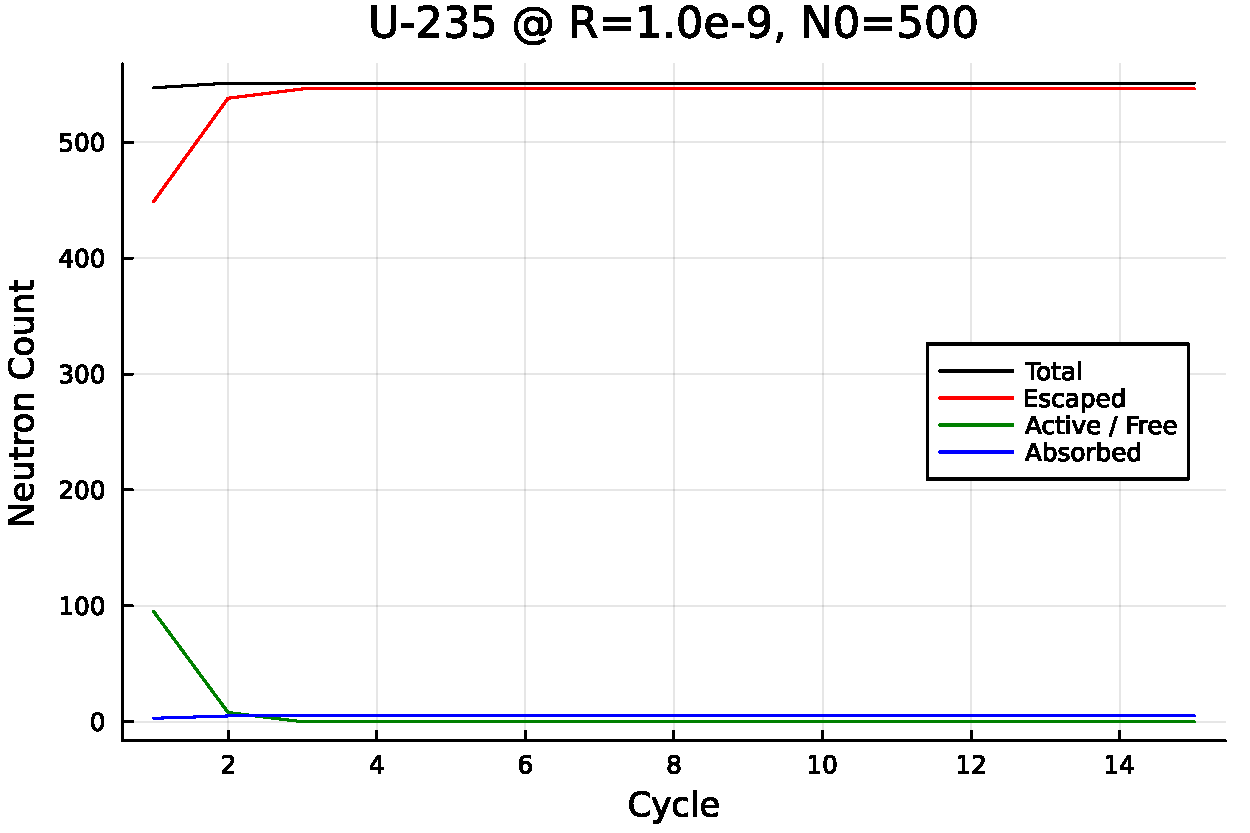
\includegraphics[scale=0.55]{imgs/neutron-count-uranium-large-sphere.pdf}
    \caption{A ``large'' sphere with radius $10^{-9}$cm, and a starting population of $500$ neutrons, run for 15 simulation 
    cycles.}
\end{figure}

\begin{figure}[h!]
    \centering
    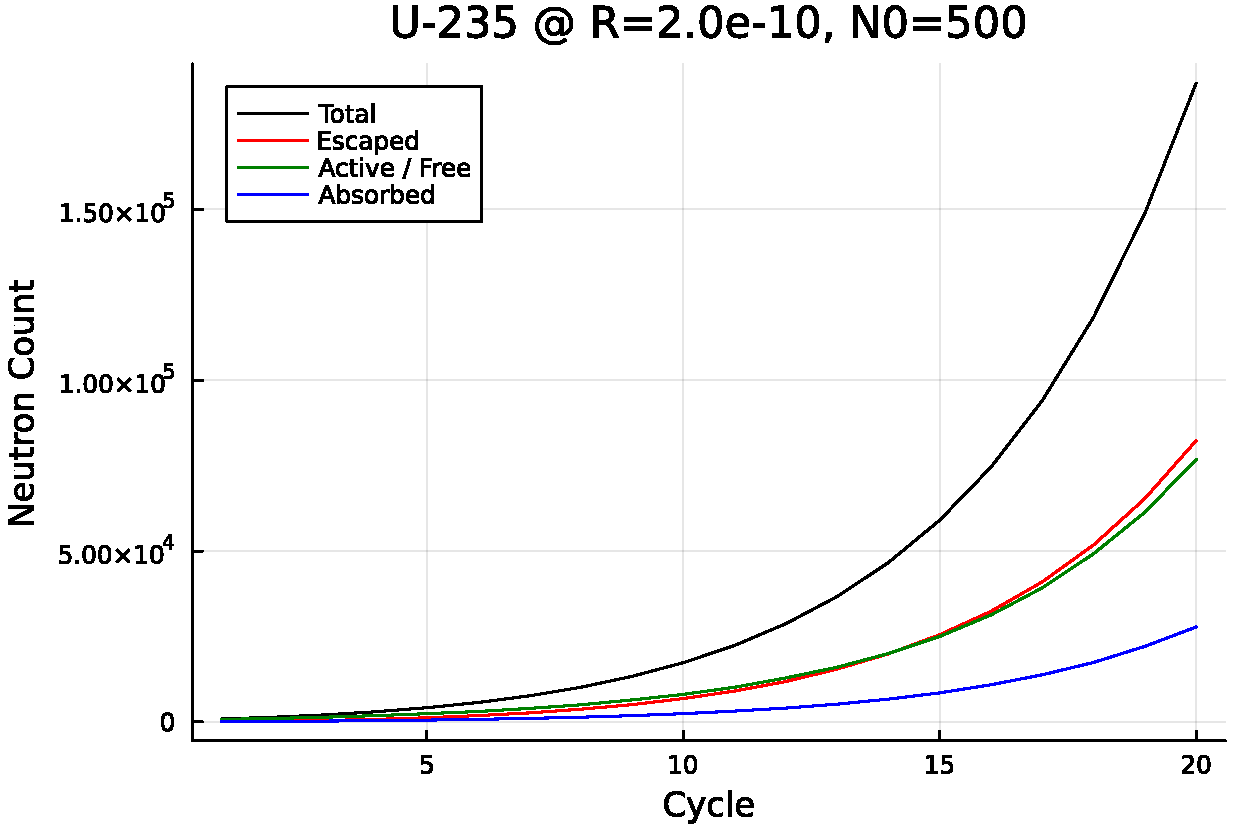
\includegraphics[scale=0.55]{imgs/neutron-count-uranium-medium-sphere-3-long.pdf}
    \caption{A ``medium'' sphere with radius $2 \cdot 10^{-10}$cm, and a starting population of $500$ neutrons, run for 20 simulation 
    cycles.}
\end{figure}\newpage

\begin{figure}[h!]
    \centering
    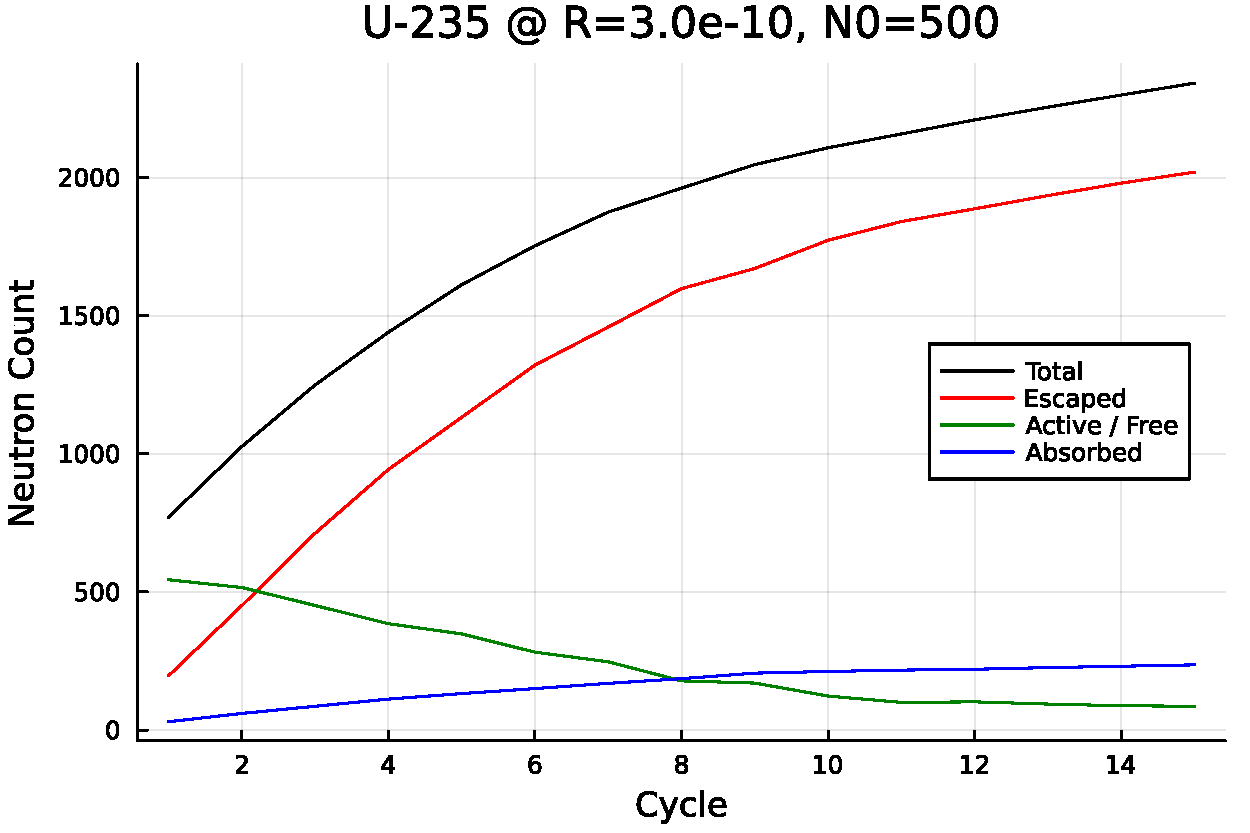
\includegraphics[scale=0.55]{imgs/neutron-count-uranium-medium-sphere-2.pdf}
    \caption{Another ``medium'' sphere with radius $3 \cdot 10^{-10}$cm, and a starting population of $500$ neutrons, run for 15 simulation 
    cycles.}
\end{figure}\newpage

\subsubsection{Critical Density Analysis}

Figures 4.1 - 4.3 show how different populations of neutrons in the medium grow under the dynamics of the system they're in. The only 
property that varies between these graphs is the radius of the sphere of Uranium in which the $500$ neutrons interact. Figure 
4.1 shows that almost all our neutrons escape almost immediately, while some are absorbed. No sustained fission reaction 
occurs in this case - we might posit that the sphere is too large (and thus the neutrons too sparse in our Uranium mass) to 
interact to a degree which encourages the production of other neutrons. This would be supported by the fact that the total population 
of neutrons remains largely unchanged from the initial count of $500$. 

This is in stark contrast to what we observe in, say, figure 4.2. Here we see sphere of smaller radius (increasing density),
and observe that our neutron population grows in what appears to be an exonential manner. Here, we are observing a self-sustaining 
fission reaction which has become super-critical. While some neutrons are still escaping, we see that the number of active neutrons 
is still growing exponentially, and so the reaction will self sustain. 

Figure 3.3 shows a more middle ground between the two. Theoretically it is possible to have a fission reaction system which is self sustaining,
without being super-critical or sub-critical. In practice, however, this is impossible as it requires a perfect balance of conditions which 
is not feasible in the real world. This figure depicts behaviour approaching that boundary, where the population of neutrons eventually decays 
to a sub-critical state, however does so at a slower rate than figure 4.1 which had a sphere of larger radius and so reached that state of 
non-reaction much faster.

We can see the relationship between radius of the sphere and the neutron population growth rate more clearly in figure \ref{uranium-total}. 

\begin{figure}[h!]
    \centering
    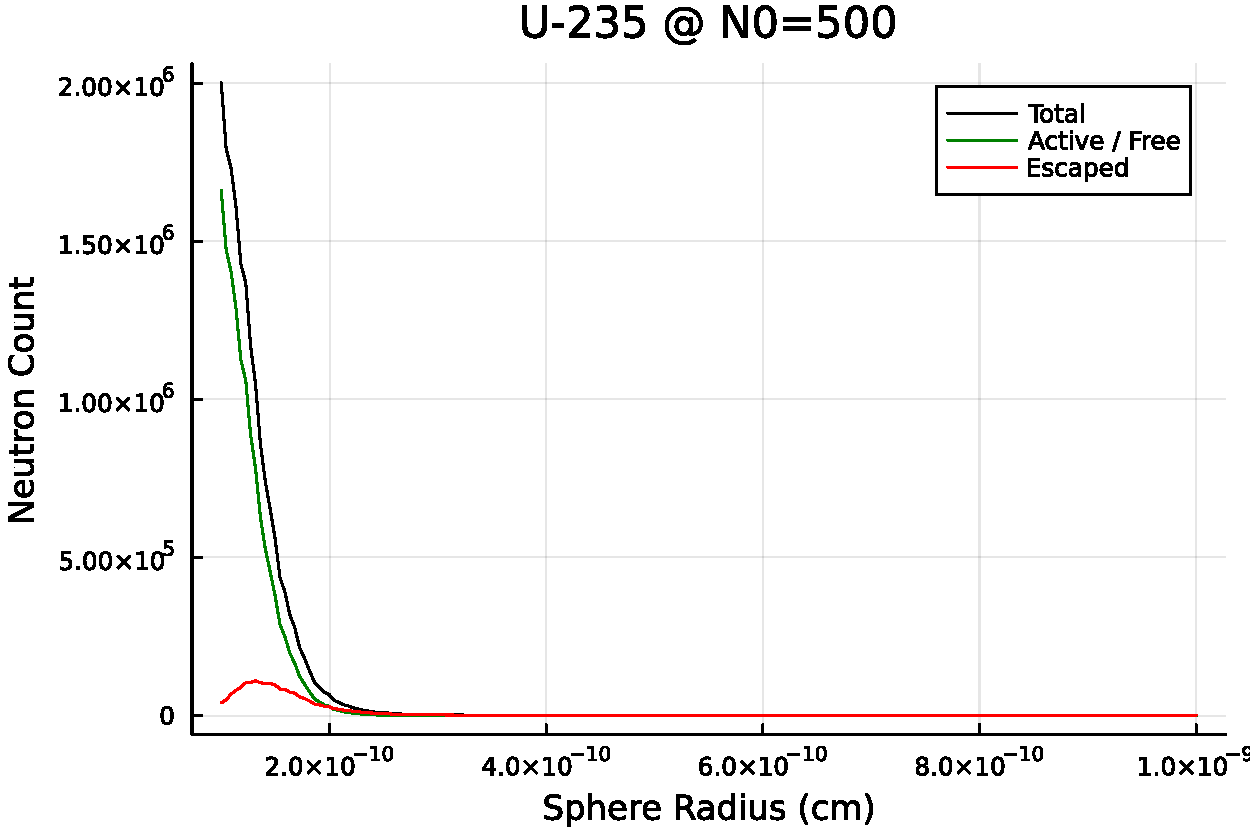
\includegraphics[scale=0.55]{imgs/radius-variation-uranium.pdf}
    \caption{Neutrons present in a mass of Uranium condensed into sphere of given radius (i.e. density is leftwards increasing in 
    the graph).}
    \label{uranium-total}
\end{figure}

There is a point (around $3 \cdot 10^{-10} \text{cm}$) for which 
a sphere of greater radius will not result in a burn up situation - i.e., the number of neutrons either remains the same or 
decreases such that the reaction fizzles out. For spheres with a radius smaller than this, however, we see an exponential rise in the amount 
of neutrons as radius decreases. This is consistent with behaviour expected from super-critical systems, that is to say, 
it identifies the critical density for Uranium (when there are that many neutrons present). As we stated in our limitations, 
the number of neutrons present is incredibly unrealistic, and so we are unable to determine from this what the actual 
critical density of Uranium might be, unfortunately. However we are still able to identify behaviour, as the system scales nonetheless.

Note that there seems to be a dip in escaped neutrons as the sphere continues to decrease in radius. This is a misnomer, and 
is actually due to floating point errors - this comes about in the calculation of the euclidean distance of a neutron from 
the origin, and as distances decrease in size these values become smaller, until the code can no longer support their precision.

\subsection{Pu-239 Simulations}

\subsubsection{Density Variation}

\begin{figure}[h!]
    \centering
    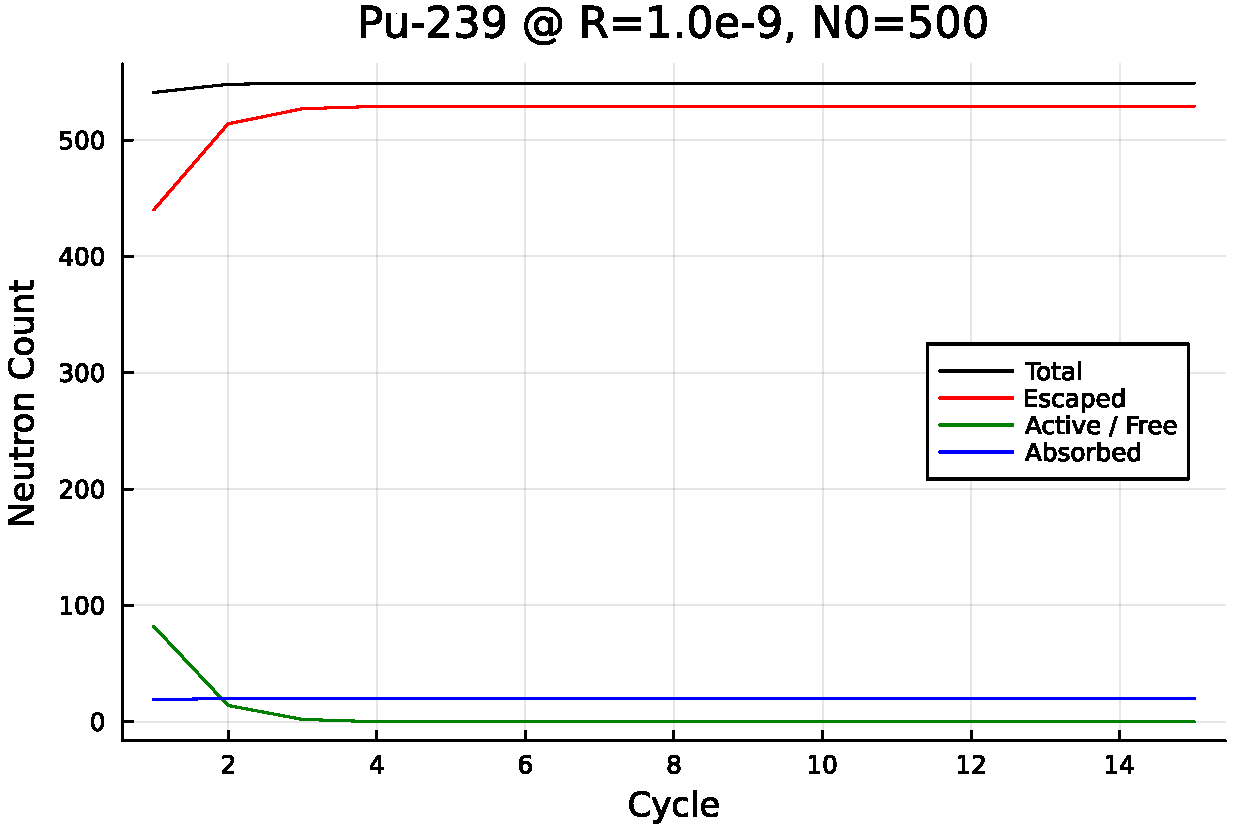
\includegraphics[scale=0.55]{imgs/neutron-count-plutonium-large-sphere.pdf}
    \caption{A ``large'' sphere with radius $10^{-9}$cm, and a starting population of $500$ neutrons, run for 15 simulation 
    cycles.}
\end{figure}

\begin{figure}[h!]
    \centering
    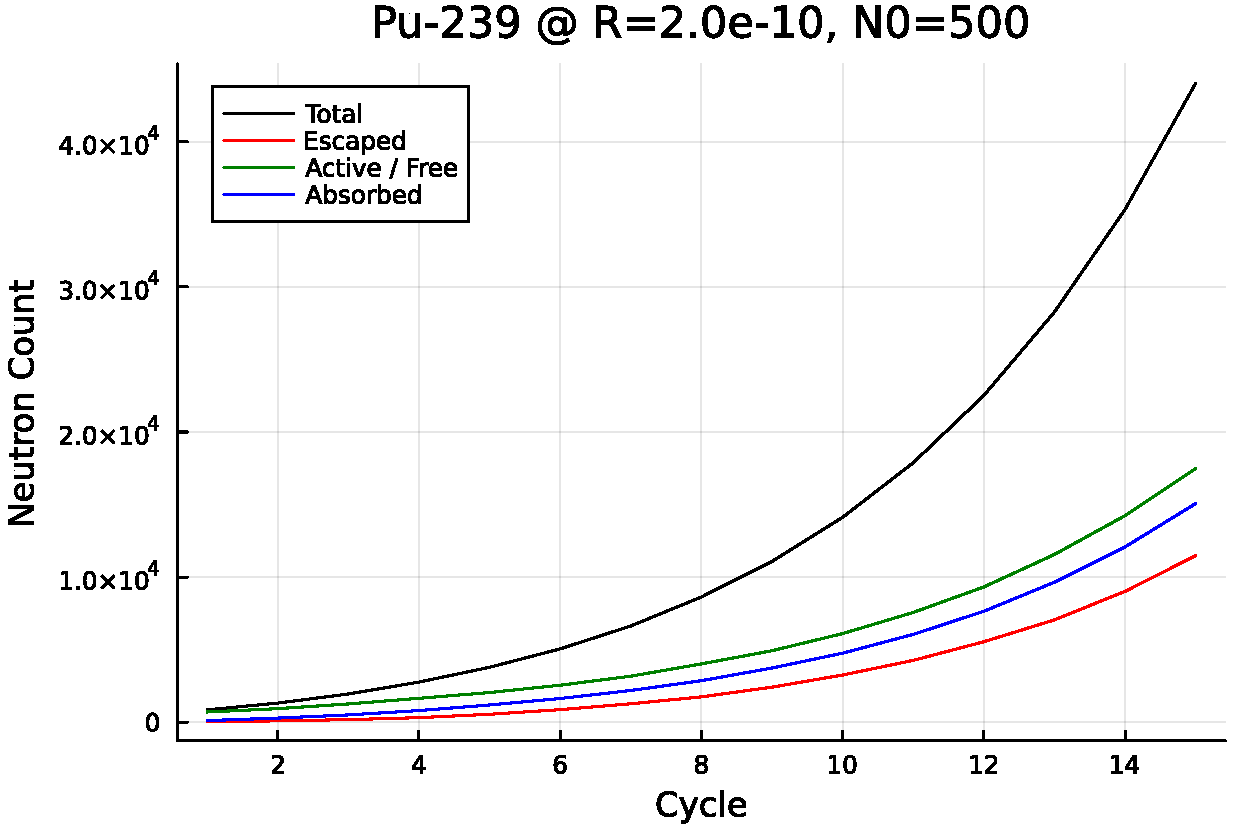
\includegraphics[scale=0.55]{imgs/neutron-count-plutonium-medium.pdf}
    \caption{A ``medium'' sphere with radius $2 \cdot 10^{-10}$cm, and a starting population of $500$ neutrons, run for 20 simulation 
    cycles.}
\end{figure}

\begin{figure}[h!]
    \centering
    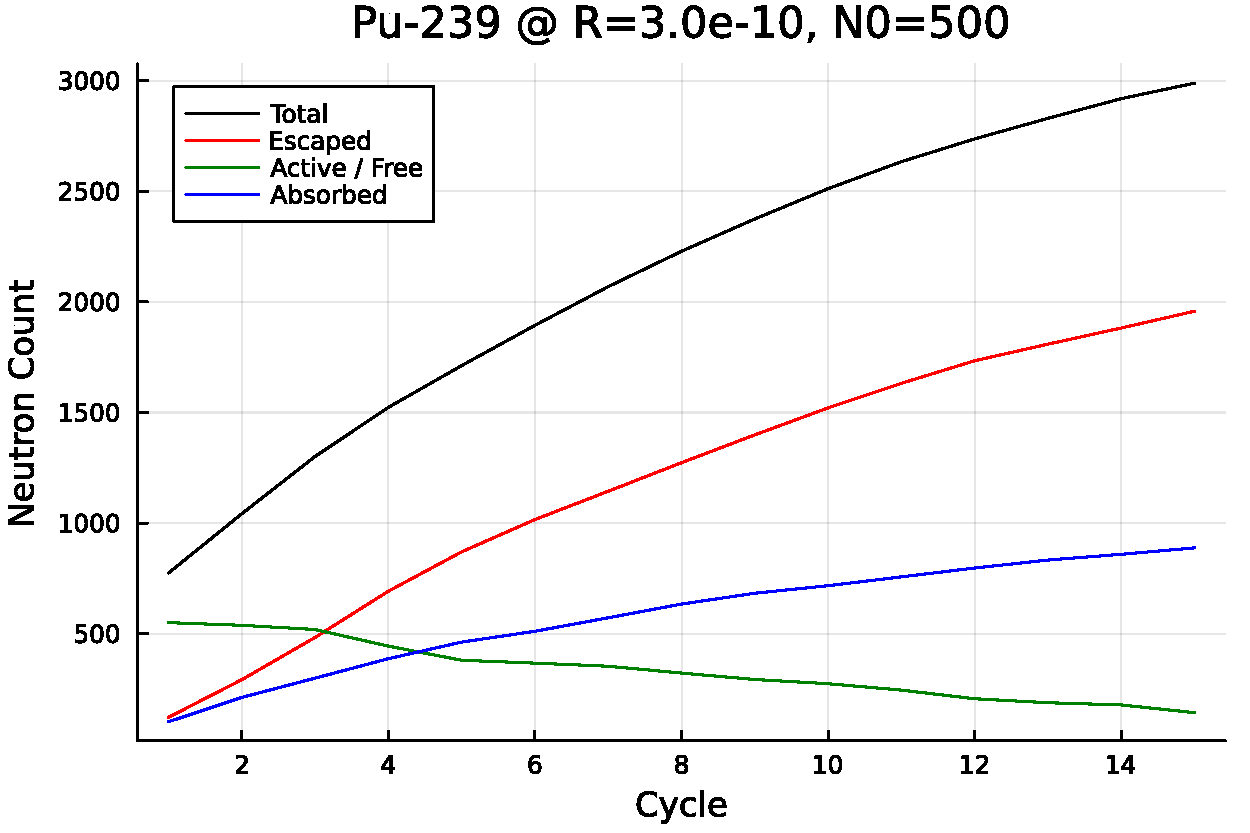
\includegraphics[scale=0.55]{imgs/neutron-count-plutonium-medium-2.pdf}
    \caption{Another ``medium'' sphere with radius $3 \cdot 10^{-10}$cm, and a starting population of $500$ neutrons, run for 15 simulation 
    cycles.}
\end{figure}\newpage

\subsubsection{Critical Density Analysis}

We largely include Plutonium in our simulations for two reasons: 1. because the bomb developed at Los Alamos had a Plutonium core, and 
it seemed only fitting to include a Plutonium simulation given the origins of the work in this; and 2. so we have something to compare the 
Uranium simulations to. 

\begin{figure}[h!]
    \centering
    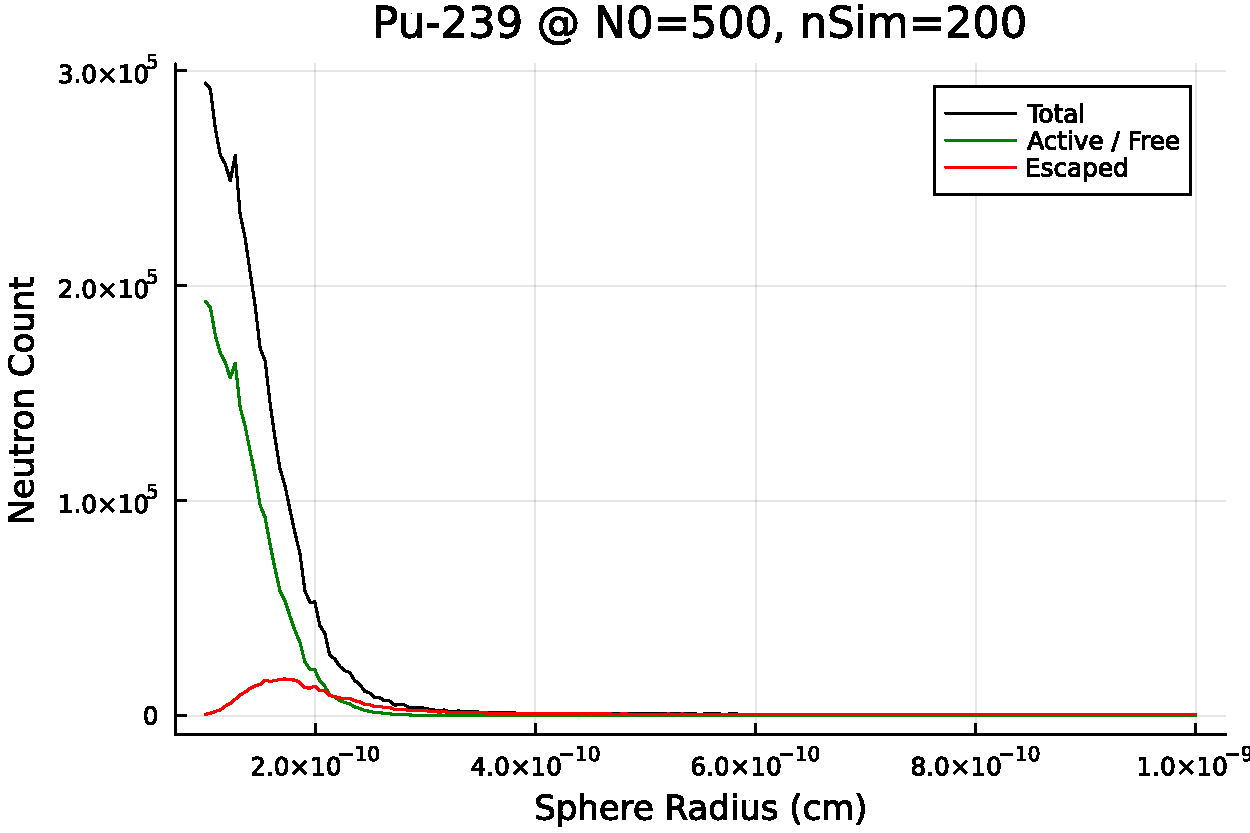
\includegraphics[scale=0.55]{imgs/radius-variation-plutonium.pdf}
    \caption{Neutrons present in a mass of Uranium condensed into sphere of given radius (i.e. density is leftwards increasing in 
    the graph).}
    \label{plutonium-total}
\end{figure}

When it comes to the Plutonium results, we see much the same behaviour as we did for Uranium, and for the same reasons. We only have 
to note that the orders to which the neutrons grow is somewhat greater for Uranium than for Plutonium. For example, for a sphere 
of radius $2 \cdot 10^{-10}\text{cm}$ Plutonium grew to a population of approximately 40000 neutrons, whereas Uranium sat 
comfortably at approximately 200000. If we recall back to our table which described the average cross section data for 
Uranium and Plutonium, we note that the average cross section values for capture and fission events are both greater for Plutonium 
than for Uranium. That is to say, a thermal neutron, on average, will have to travel farther through a Plutonium medium in order 
to experience a fission event, than it would if it were in a Uranium medium. Additionally, from these values, the probability 
of a fission reaction occurring sits at approximately $78$\% for Plutonium, whereas it sits at approximately $85$\% for Uranium.
Thus, we would expect there to be more fission reactions for a Uranium medium, and thus more opportunity for neutron development. The 
trend therefore is similarly consistent for comparisons between materials.
\include{further_work}
\section{Conclusions}

\subsection{What did we achieve?}

\subsection{Future work?}


\textbf{Neutron Reflector} \\
When it comes to nuclear reactors, one goal of your system is to keep the neutron count in equilibrium so as to ensure a sustained 
reaction that doesn't grow too quickly and lead to super-critical conditions (i.e., an explosion). However, there is a case 
where you would want this rapid growth in reactions - in the case that you want an explosion! Whereas nuclear reactors have 
devices designed to regulate neutron energy and count, a nuclear bomb has the opposite goal. However, one of the larger 
causes for loss of neutrons is that they simply leave the medium you are trying to contain them within. As such, one 
method often used (which was invented at Los Alomos for the Trinity test) is to have a ``neutron reflector''. This is an 
outer casing around your bomb which biases the reflection angle when it comes to elastic scattering collision events for neutrons 
operating within the bounds of the bomb medium. This decreases the loss of neutrons to the environment, and thus maintains 
density of neutrons for longer, making it easier for a sustained and super-critical fission reaction to develop. One such extension 
could be then to include support for such a structure into the simulation, and to observe how it affects the critical density of both 
isotopes. 

\noindent\textbf{Other Fission Reactions} \\
Currently in the simulation, if a neutron's collision is deemed to produce a fission event, we only support the case that one neutron 
is ejected from the atom our neutron has collided with. This is referred to as an (n,2n) reaction. However, it is possible 
for more outputs -- an (n,3n) reaction is possible for example, where two excess neutrons are ejected from the target atom. This would 
increase the number of neutrons present in the medium, and is more physically accurate. 

\noindent\textbf{More Precise Scattering Variants} \\
Currently only in-elastic scattering is supported, however in real kinetic dynamics, this is infeasible. When a neutron collides 
with an atom, it should be affected by the momentum of the atom, instead of randomly picking a direction to head in next. Similarly, 
for cases of fission events, the resulting neutron should be affected by the 

\noindent\textbf{Neutron Energy Distributions} \\
In simplifying our model to assume a uniform, averaged neutron energy, we ignore many effects. For example, there is a significant difference 
between mean free-paths for thermal and fast neutrons, and each have their own purpose. For example, in a nuclear reactor you wish to have 
more thermal neutrons as they caise fission reactions over longer time scales, whereas fast neutrons will result in more fission events 
in shorter periods. Some analytic approximations to energy distributions for neutrons within medium are available, and these could be incorporated 
into our model to more accurately represent the behaviour of neutrons. This would well be accompanied by a more precise implementation 
of scattering methods as described above, as they are also somewhat dependent on energies of participating neutrons.

\noindent\textbf{Reaction Medium Geometries} \\
We could also support different geometries. Currently we assume a sphere, which is quite simplistic. Some more academic 
structures such as a cube would not be difficult to implement and provide some interesting analytics, however some 
other geometries such as a cylinder could be useful for simulations on reactor cores for example.


\bibliography{bibliography}
\bibliographystyle{plain}

%%% End document
\end{document}
